%%%%%%%%%%%%%%%%%%%%%%%%%%%%%%%%%%%%%%%
%----------------------------------------     算法     ---------------------------------------%
%%%%%%%%%%%%%%%%%%%%%%%%%%%%%%%%%%%%%%%
\chapter{属性网络中的增量图表征算法}
\section{引言}
图表征算法今年来吸引了大量关注,在图表征算法中一种朴素的思想是保留网络中节点的接近度,在上一章中本文提出了一种保留高阶接近度的网络表征学习算法,并相应地提出了增量场景下的图表征算法。可是,上一章的算法忽略了真实网络的特性,即网络中节点本身具有丰富的节点属性。网络除了拓扑结构信息以外,节点本身的属性也会影响影响节点分类和链路预测等的结果,比如,社交网络两个没有连接的用户节点,如果拥有越多共同的兴趣爱好或话题,那么成为好友或互相关注的可能性就会越大,因为用户节点除了通过物理连接形成在线社区以外,还会分享观点并评论而形成一些话题圈;相反没有共同兴趣爱好或话题但存在连接的用户节点则会使关系强度越变越弱。从现实的应用中可以看出,在有节点属性信息的网络中(后文将统一称为属性网络),节点的属性信息扮演着非常重要的角色。

在属性网络中,直接将网络中节点的属性作为节点表征向量的附加特征,再将组合得到的表征向量作为机器学习任务的输入是可行的,但是存在两个问题:1.对于节点特征为稀疏高维特征时,直接附加特征进行组合的方法会使得学习任务复杂度变高;2.忽略了网络结构与节点属性之间的耦合信息,节点属性特征之间的相关性被忽略。因此,不同于普通的网络图表征算法,属性网络的图表征算法需要平衡好网络结构相似度和节点属性之间的关联\cite{huang2017label}。

本章将提出一种属性网络中的图表征算法框架,以节点属性特征为主体,提出基于相似度的属性表征方法,根据分析对比模型的变化,提出增量场景下的相似度降维方法。

\section{问题描述}
假设一个无向属性网络$G=\{\textbf{A}, \textbf{H}\}$,其中\textbf{A}为网络的邻接矩阵,\textbf{H}为网络中节点的属性矩阵,且属性矩阵 $\textbf{H}\in R^{|V|\times d}$,$d$为节点属性特征的维数。属性网络图表征算法可视为寻找一个映射函数来表征网络中的每个节点:
\begin{equation}
f_G: \textbf{A}, \textbf{H} \rightarrow \textbf{X} \in R^{|V| \times k} \qquad s.t.\quad k<<|V|
\end{equation}

区别于上一章对静态场景和增量场景下网络结构的表征学习,本章研究对象为节点属性特征,基于节点属性的相似度对属性网络进行表征学习。下面将分别对静态场景和增量场景下的的属性网络表征学习进行介绍和分析。

\section{静态场景下属性网络表征学习}
在属性网络中对节点属性的表征学习不同于对节点属性进行直接的数据降维,前者更加关注节点属性之间的相似度关系,同时网络结构本身的信息可以对节点属性表征过程进行修改和调整,在这个过程中一个重要过程是通过节点属性特征计算相似度,下面将介绍三种相似度计算方法:
\definition{余弦相似度}:

 余弦相似度通过计算两个向量的夹角来计算向量之间的相似度,夹角越小,则相似度越大,余弦相似度的取值范围在[-1,1], 如果相似度为负2,则两个向量负相关。在计算两个节点属性$\textbf{H}_i, \textbf{H}_j$相似度时,余弦相似度记为$Sim_{cos}$,表达式如下:
\begin{equation}
	Sim_{cos}(H_i, H_j) = \frac{H_i \cdot H_j}{|H_i||H_j|}
\end{equation}
在实际场景中,余弦相似度存在不足,当不同特征的尺度不一致时容易使得其中一维特征就产生较大的影响,比如有大部分特征尺度为0到1,其中有一维特征的量级为1000,那么其他特征的对相似度计算的影响就很小了,因此在实际应用场景中经常会对特征进行归一化。

\definition{皮尔逊相似度(Pearson Correlation Coefficient)}

皮尔逊相似度是基于余弦相似度的改进,用来衡量两个变量之间的线性关系,同样的皮尔逊相似度的取值范围为[-1,+1],两个节点属性$\textbf{H}_i, \textbf{H}_j$的皮尔逊相似度记为$Sim_{pcc}$,计算皮尔逊相似度的方法为:
\begin{equation}
	Sim_{pcc}(H_i, H_j) = \frac{\sum_{x=1}^n(\textbf{H}_{i,x}-\bar{\textbf{H}}_i)(\textbf{H}_{j,x}-\bar{\textbf{H}}_j)}
	{\sqrt{\sum_{x=1}^n \textbf{H}_{i,x} ^2 }\sqrt{\sum_{x=1}^n \textbf{H}_{j,x} ^2 }}
\end{equation}


\definition{KL散度}

KL散度又称为相对熵,用来衡量两个随机变量之间之间的距离,前文在LINE算法中提及过。不同于前面的相似度计算方法,两个向量之间的KL散度是距离函数,也即向量越相似,KL散度越小。KL散度为非负值,两个节点属性$\textbf{H}_i, \textbf{H}_j$的KL散度记为$d_{kl}$,计算KL散度的方法为:
\begin{equation}
	d_{kl}(H_i|H_j) = \sum_{x=1}^n H_{i,x}\log{\frac{H_{j,x}}{H_{i,x}}} 
\end{equation}
从上式中可以看出KL散度具有不对称性,也即:
\begin{equation}
d_{kl}(H_i|H_j) \ne d_{kl}(H_i|H_j)
\end{equation}
因此基于KL散度,本文采用基于KL散度改进的相似度方法,记为$Sim_{kl}$:
\begin{equation}
Sim_{kl}(H_i, H_j)=\left\{
\begin{array}{ccl}
\frac{1}{d_{kl}(H_i|H_j)+d_{kl}(H_j|H_i)}       &      & d_{kl}(H_i|H_j)\ne 0\\
1     &      & d_{kl}(H_i|H_j)=0
\end{array} \right.
\end{equation}

三种相似度各有不同的优势和劣势,在后文中将以算子$Sim(\cdot)$对同一表示上述三个相似度计算方法。通过相似度计算可以得到节点属性特征的相似度矩阵$\textbf{S}^H$,基于相似度矩阵提出表征算法。
\begin{figure}[!ht]
	\begin{center}
		{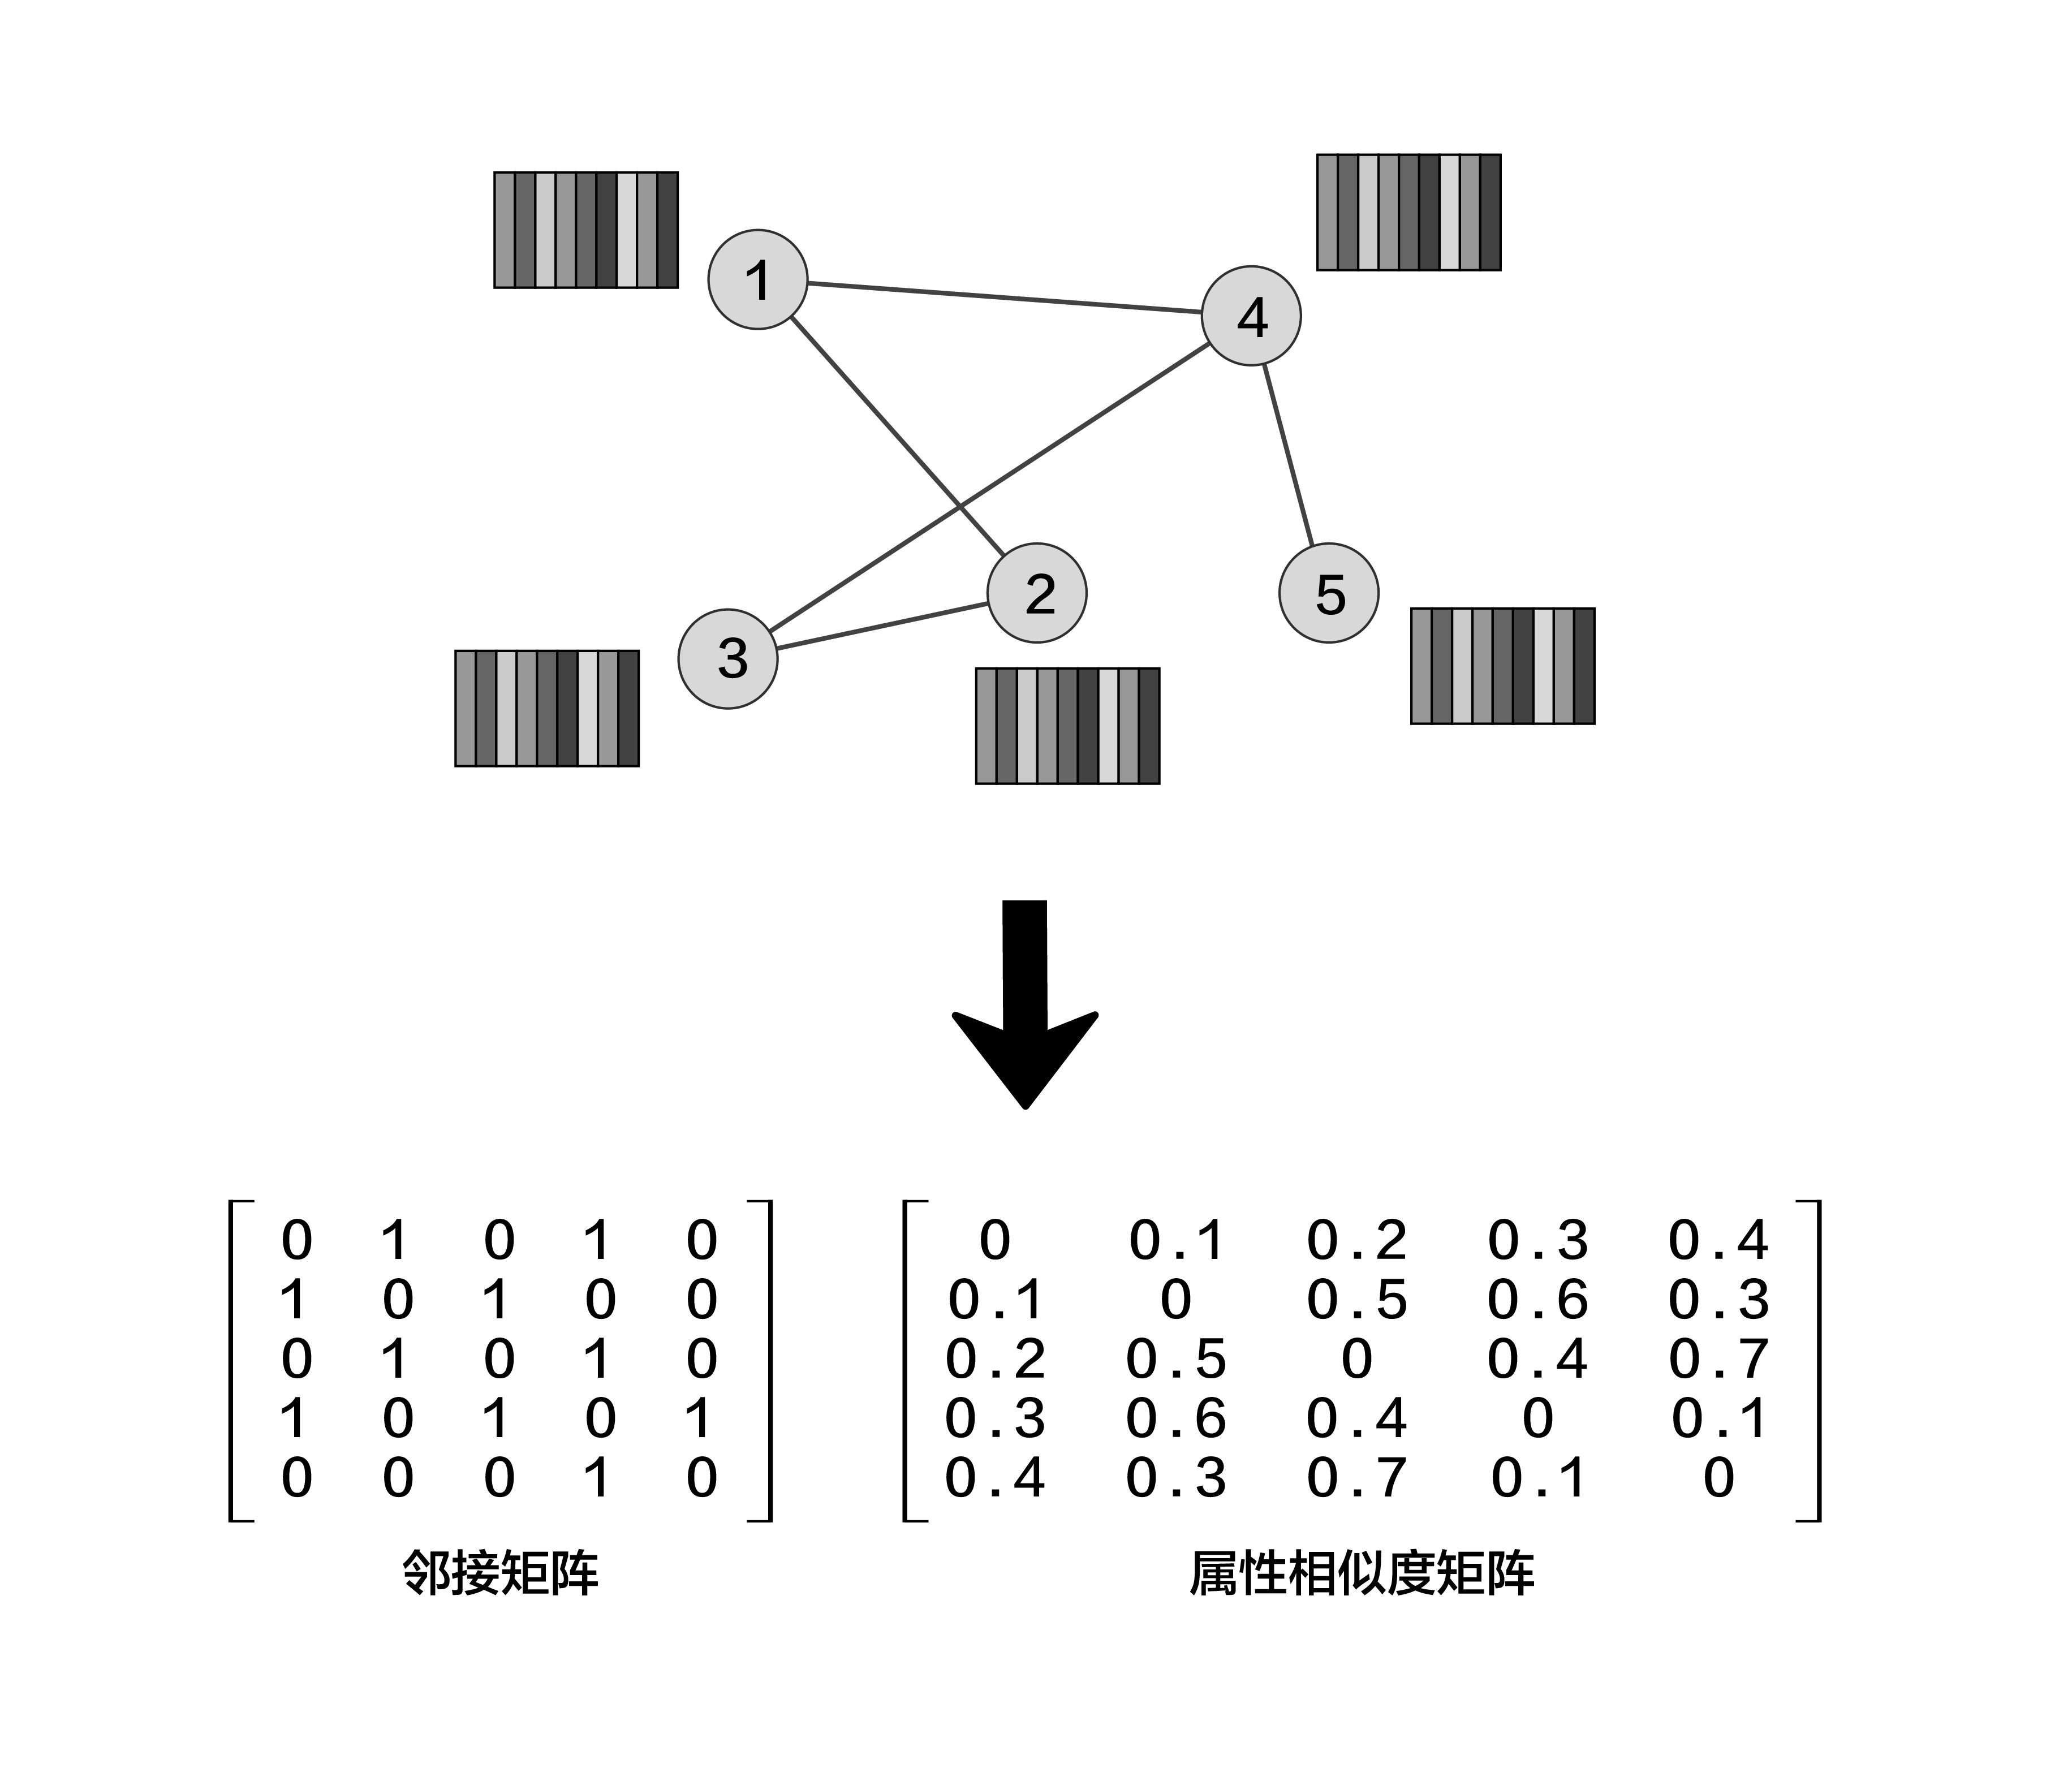
\includegraphics[width=5in]{figures/attributed_matrix.png}}
		\caption{邻接矩阵和属性相似度矩阵系数性对比}
	\end{center}
\end{figure}

不同于节点邻接矩阵或其他相似度矩阵,属性特征的相似度矩阵中并非稀疏矩阵,矩阵中大部分为非零元素,在此提出一种基于图分解的方式进行属性表征学习。
\subsection{基于图分解的相似度表征学习}
图分解(Graph Factorization)\cite{ahmed2013distributed}是ahmed等在2013提出的一种在分布式场景下的图表征方法,用于在大网络中快速有效的计算节点向量表征。在图分解中为了设计的灵活性直接采用表征向量的点积用来表征节点的接近度,也即对于连边$A_{ij}$通过表征向量点积来表征$<X_i, X_j>$,另外为了保证在数据量比较小的时候,模型仍保持较好效果,因此在目标函数中引入了正则项进行优化,模型的目标函数如下:
\begin{equation}
	\min \quad f(A, X)=\frac{1}{2} \sum_{(i,j)\in E}(A_{ij}-<X_i, X_j>)^2+\frac{\lambda}{2}\sum_i|X|^2
\end{equation}
对上述目标函数求极值,采用梯度下降的方式。函数$f$对于$X_i$的梯度计算为:
\begin{equation}
\frac{\partial f}{\partial X_i} = -\sum_{j\in N(i)} (A_{ij}-<X_i,X_j>)X_j+\lambda X_i
\end{equation}
因此对于网络中任意一条两边$(i,j)\in E$,上式值等于:
\begin{equation}
	-(A_{ij}-<X_i, X_j>)X_j - \lambda X_i
\end{equation}
进一步对任意$X_i$,则可以通过梯度下降公式进行更新:
\begin{equation}
	X_i = X_i + \eta [(A_{ij}-<X_i, X_j>)X_j - \lambda X_i]
\end{equation}
其中$\eta$为迭代中设置的步长。在图分解算法中邻接矩阵$A$通常不是半正定矩阵,即使节点表征向量维度为$|V|$,损失函数也不会降到0。通过对图分解算法的计算复杂度分析可以发现,算法对网络中连边进行遍历来进行迭代优化,计算复杂度为$\mathcal{O}(|V|)$。

于是,在属性网络中,基于图分解的相似度表征算法转化为利用节点表征向量的点积来描述节点之间属性的相似度。对于节点$i$,记属性表征后的节点属性表征向量为$\textbf{X}_i^H$,通过节点属性计算的相似度矩阵为$\textbf{S}^H$,则相似度表征算法的优化函数为:
\begin{equation}
\min \quad f(\textbf{S}^H, \textbf{X}^H)=\frac{1}{2} \sum_{i\ne j}(\textbf{S}^H_{ij}-<\textbf{X}^H_i, \textbf{X}^H_j>)^2+\frac{\lambda}{2}\sum_i|\textbf{X}^H|^2
\end{equation}
同样采取梯度下降进行优化求解,对于任意$i\ne j$,迭代更新公式为:
\begin{equation}
	\textbf{X}^H_i = \textbf{X}^H_i + \eta [(\textbf{S}^H_{ij}-<\textbf{X}^H_i, \textbf{X}^H_j>)\textbf{X}^H_j - \lambda \textbf{X}^H_i]
\end{equation}
通过不断地迭代使得表征向量趋于稳定,在达到迭代终止条件时,算法终止。

下面将给出相似度表征算法SR1(Similarity Representation version1)的过程描述。
\subsection{SR1算法描述}
给定无向属性网络$G=\{\textbf{A}, \textbf{H}\}$和属性表征向量维数$k$,其中$\textbf{H}$表示网络的节点属性矩阵,即$\textbf{H}\in R^{|V|\times d}$,$d$为节点属性特征维数,SR1算法将得到图$G$属性表征矩阵$\textbf{X}^H\in R^{|V|\times k}$,详细算法过程见\textbf{算法4.1}。
\begin{figure}[htb]
	\centering
	\begin{minipage}{.7\linewidth}
		\begin{algorithm}[H]
			\small
			\caption{SR1算法}
			\begin{algorithmic}[1]
				\Require
				\Statex $\textbf{H}$ :节点属性矩阵$R^{|V|\times d}$
				\Statex $k$ : 属性表征向量维数
				\Statex $\epsilon$:迭代终止误差
				\Ensure
				\Statex $\textbf{X}^H$ :属性表征向量矩阵
				\Statex
				\State \textbf{for} i in range(\textbf{H}.shape[0]):
				\State \quad \textbf{for} j >i:
				\State\qquad	$\textbf{S}^H_{ij}=\textbf{S}^H_{ji} = Sim(H_i, H_j)$
				\State \quad \textbf{end for}
				\State \textbf{end for}
				\State 随机初始化临时属性表征向量$\textbf{X}^{H\prime}\in R^{|V|\times k}$
				\State $t \leftarrow 1$
				\State do:
				\State \quad $\textbf{X}^H\leftarrow\textbf{X}^{H\prime}$
				\State\quad \textbf{for} i in range(\textbf{H}.shape[0]):
				\State\qquad \textbf{for} j in range(\textbf{H}.shape[0]) and $i\ne j$:
				\State\quad \qquad $\eta \leftarrow \frac{1}{\sqrt{t}}$
				\State\quad \qquad $t\leftarrow t+1$
				\State\quad \qquad $\textbf{X}^H_i \leftarrow \textbf{X}^H_i + \eta [(\textbf{S}^H_{ij}-<\textbf{X}^H_i, \textbf{X}^H_j>)\textbf{X}^H_j - \lambda \textbf{X}^H_i]$
				\State \qquad \textbf{end for}
				\State \quad \textbf{end for}
				\State 当$|\textbf{X}^{H\prime}-\textbf{X}^H|^2<\epsilon$停止迭代
				\State 返回 $\textbf{X}^H$
			\end{algorithmic}
		\end{algorithm}
	\end{minipage}
\end{figure}

第1-5行:在算法开始时,要根据属性矩阵$\textbf{H}$,计算节点间的属性相似度,得到矩阵$\textbf{S}^H$,相似度计算方法可采用余弦相似度、皮尔逊相似度和基于KL散度改进的计算方法得来。

第6-17行:随机初始化表征向量矩阵$\textbf{X}^H$,设置迭代时间步t,用来更改迭代步长$\eta$,其中迭代步长 $\eta = \frac{1}{\sqrt{t}}$,随着迭代次数递减。对相似度矩阵中每一个非零元素(除对角线)进行一个梯度下降过程(Line 14),按第14行的方式更新节点的属性表征向量。

\subsection{SR1算法分析}
SR算法以节点特征属性矩阵作为输入,需要计算所有节点对之间的属性相似度,计算复杂度为$\mathcal{O}(|V|^2)$;再以梯度下降方式对目标函数进行优化求解,计算复杂度为$\mathcal{O}(|V|^2)$,可以得出SR算法的复杂度为$\mathcal{O}(|V|^2)$。对于SR算法的优化思路考虑在属性相似度计算是考虑网络节点之间的相互关系,用来简化计算,比如计算共同邻居矩阵$S_{CN}$,对非零元素对应的行列标号所对应的节点计算相似度,从而降低复杂度。

\subsection{优化算法SR}
从前面的算法流程和算法分析可以看出,上述的SR1算法存在两个问题:
\begin{itemize}
	\item 计算复杂度高。从前文的算法复杂度分析,得知计算复杂度为$\mathcal{O}(|V|^2)$,其中$|V|$为网络中节点数,模型在网络节点规模较大时资源消耗较大,
	\item 没有利用结构信息。前文算法SR1的输入为属性网络矩阵,不包含网络结构信息,属性网络表征学习的特点没有体现,也即没有融合节点属性和网络结构。
\end{itemize}
\begin{figure}[!ht]
	\begin{center}
		{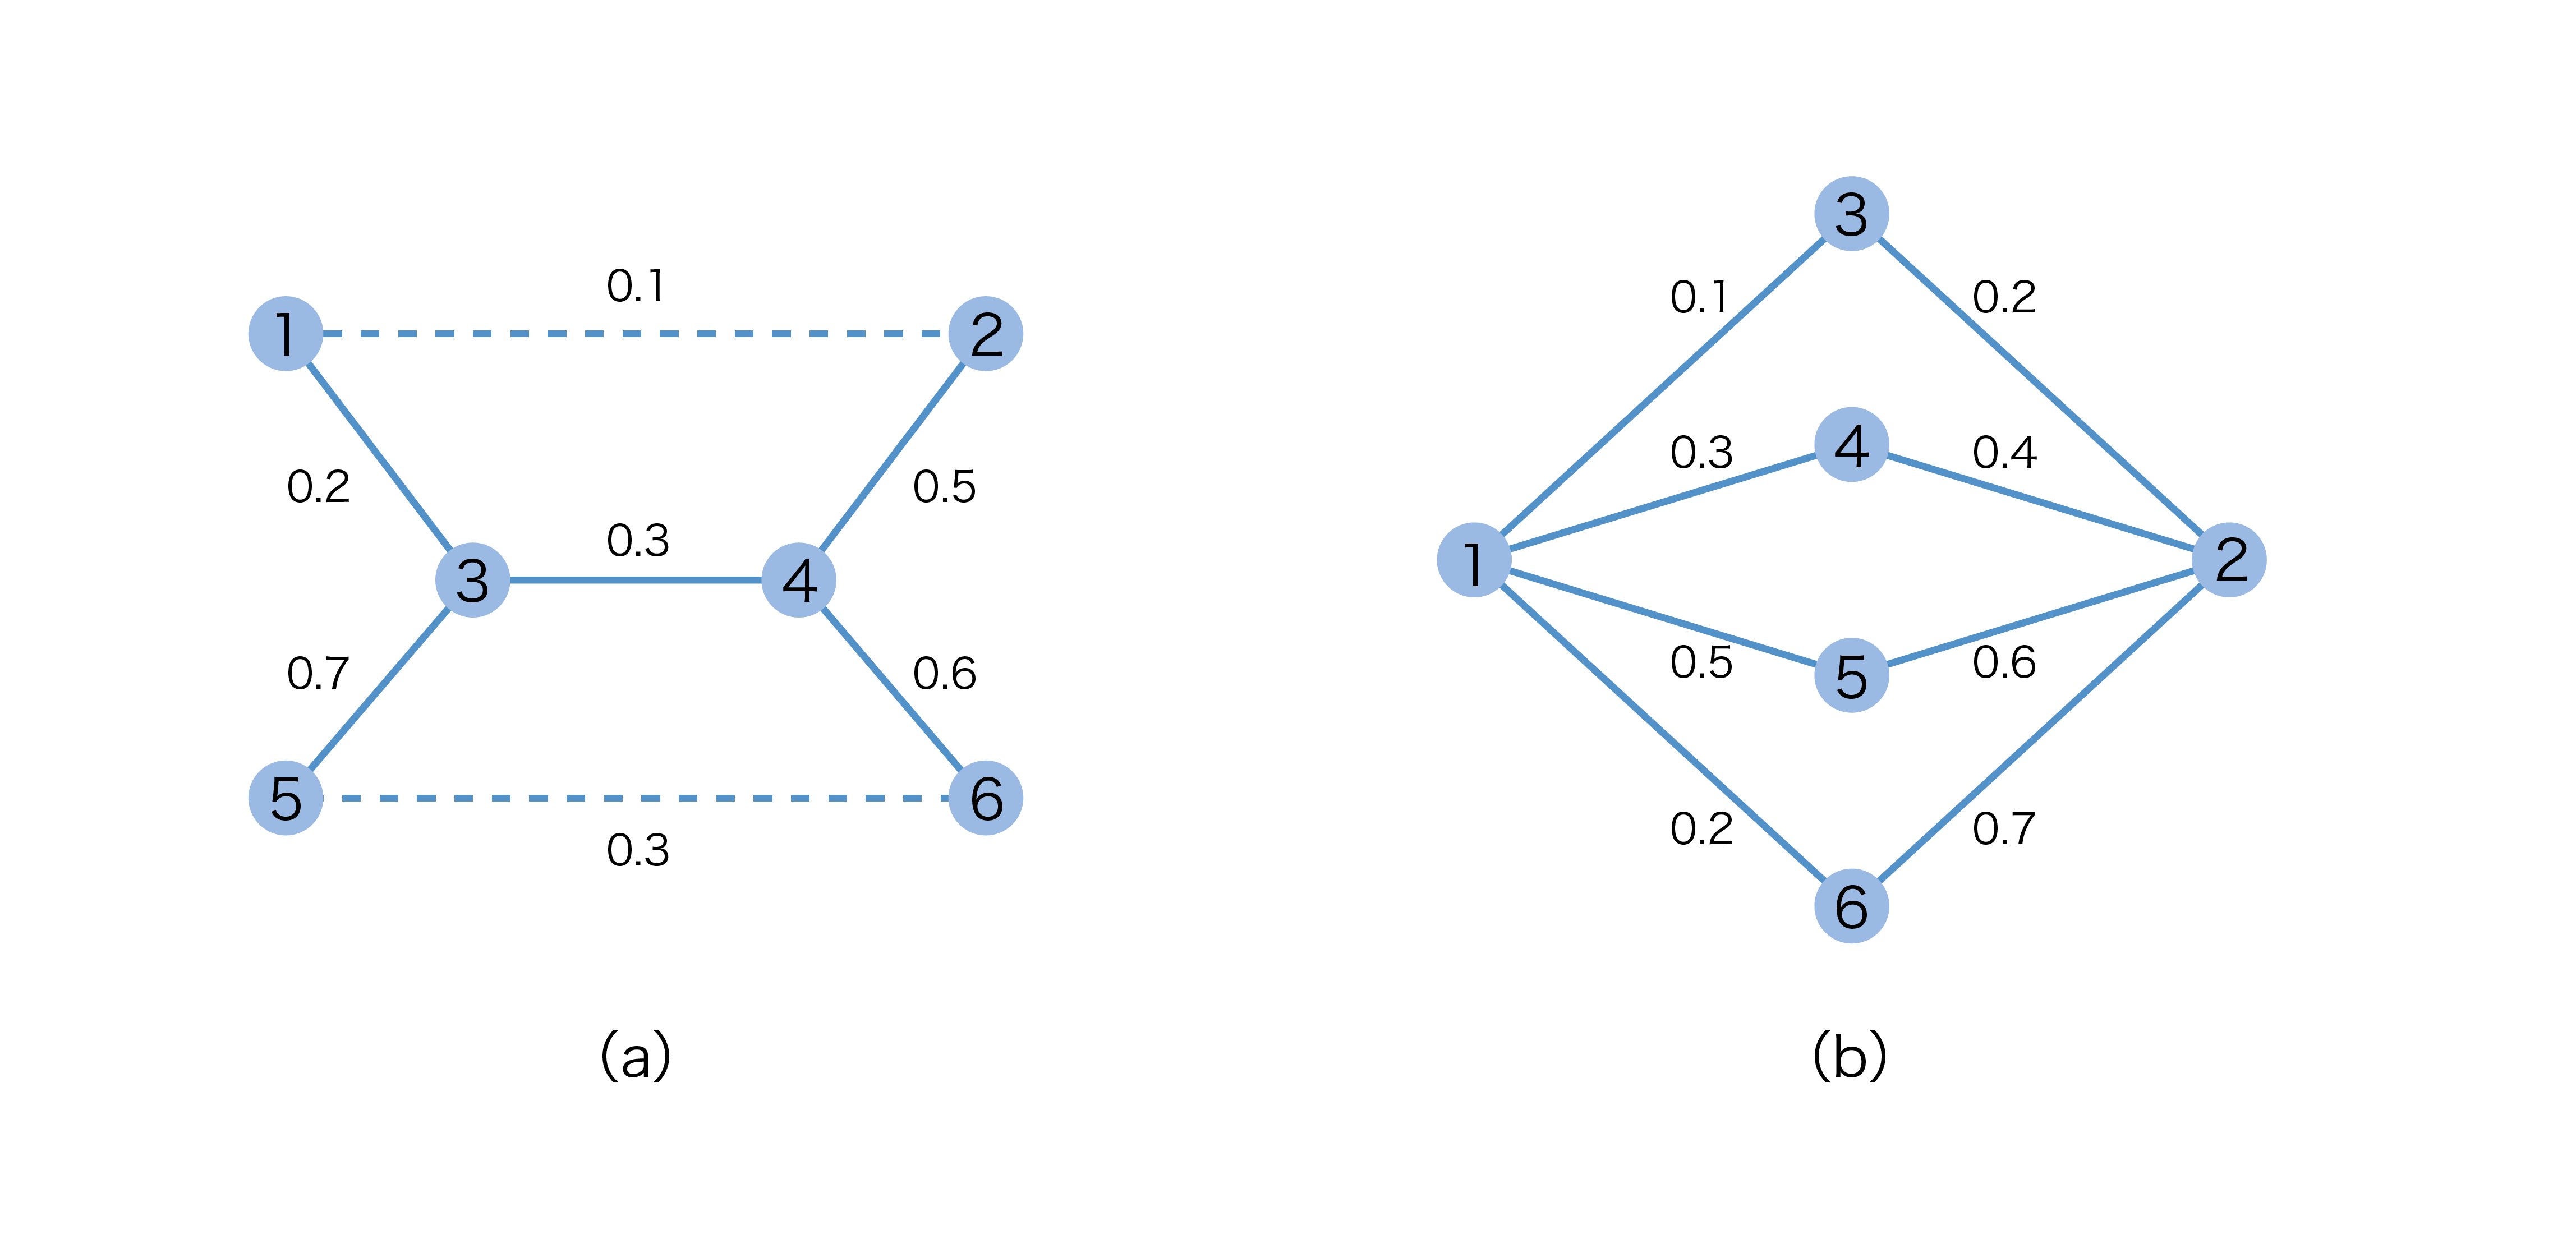
\includegraphics[width=5in]{figures/similar_opt.png}}
		\caption{网络中的属性相似度计算方法}
	\end{center}
\end{figure}
在实际网络场景中,对网络全体的节点对$(i,j)$计算基于节点属性的相似度是没有必要的。在网络中存在社区效应,节点偏向于连接社区内的节点,同一个社区内节点相互路径很短,反之,如果在网络中节点之间的路径过长则节点对建立关系的可能性也很低,进一步地,对于节点对之间网络路径过长,即使属性相似度非常高,也不会对网络本身产生影响。比如,在社交网络中,不同的人都存在亲友圈,在亲友圈中扮演相同角色的用户节点属性相似度会很高,在不存在间接共同好友的情况下,这些用户节点之间建立连接或社区的可能性较低。


\section{增量场景下属性网络表征学习}
前面一节提出了基于图分解的相似度表征方法来对节点属性特征进行表征学习,同时基于属性表征学习的缺点提出了改进算法SR。值得注意的是,真实应用中的网络往往是存在动态变化的,对于传统的特征降维过程而言,对动态增加的样本进行降维表征具有一定的挑战。





%%%%%%%%%%%%%%%%%%%%%%%%%%%%%%%%%%%%%%%
%----------------------------------------     本章小结     ---------------------------------------%
%%%%%%%%%%%%%%%%%%%%%%%%%%%%%%%%%%%%%%%
\section{本章小结}
